\section{Widzenie przez horyzont (Bartosz Strzelecki)}
Efekt został osiągnięty poprzez zmodyfikowanie potoku renderowania w taki sposób, że w zależności od wartości w buforze głębi jest wykorzystywany inny shader.
W tym przypadku, jeżeli sfera jest przysłonięta przez ścianę jest ona narysowana w przeciwnym wypadku jest uruchamiany pusty shader.
"Unity domyślnie sortuje obiekty na podstawie odległości od kamery. Tak więc
w miarę zbliżania się obiektu do kamery, będzie on rysowany nad wszystkimi obiektami znajdującymi się dalej od kamery.
W większości przypadków sprawdza się to dobrze podczas tworzenia gier, ale
znajdą się sytuacje, w których będziemy chcieli mieć większą kontrolę nad sortowaniem obiektów na scenie. Używając bloku Tags{} możemy kontrolować to sortowanie.
Unity udostępniło nam kilka domyślnych kolejek renderowania, z których każda ma unikalną wartość, którą
kieruje Unity, kiedy należy narysować obiekt na ekranie. Te wbudowane kolejki renderowania
o nazwach Background, Geometry, AlphaTest, Transparent i Overlay nie zostały stworzone arbitralnie; w rzeczywistości służą one celowi, jakim jest ułatwienie nam życia podczas
pisania shaderów i interakcji z rendererem czasu rzeczywistego."\cite{shaderscookbook}. Wykorzystując ten mechanizm
możliwe jest uzyskanie efektu widzenia postaci gracza przez horyzont.

Po naciśnięciu przycisku E następuje zagranie animacji opisanej wzorami $ w(t, offset) = 1.1 \times 2.1^{-\left(\frac{{\left(\sin(t) + 1 - 0.4 - \text{{offset}}\right)^2}}{{0.02}}\right)} $
oraz $ w(t, 0) - w(t, -0.2) + w(t, -1) - w(t, -1.2) $. Od podanych funkcji zależy przeźroczystość, jak i natężenie efektu Fresnela. 

\begin{figure}[h]
    \centering
    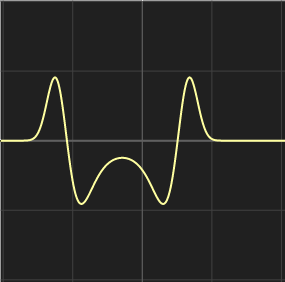
\includegraphics[width=0.25\textwidth]{images/g}
    \caption{Wykres przedstawiający funkcję opisującą zachowanie efektu Fresnela w animacji markera}
\end{figure}



\begin{lstlisting}[caption=Fragment shadera odpowiedzialny za animację]
fixed4 frag (v2f i) : SV_Target
{
  float t =  6.2 * _Progress - 0.6;
  fixed4 pattern = tex2D(_PatternTex, i.uv + _Speed *t);
  float fresnelInfluence = dot(i.worldPos, i.viewDir);
  float saturatedFresnel = saturate(1 - fresnelInfluence);

  float g = w(t, 0) - w(t, -0.2) + w(t, -1) - w(t, -1.2);
  float4 color = pow(saturatedFresnel, g * _FresnelPow) * (_Color * _ColorIntensity) * pattern;
  color.a *= dot(i.worldPos, i.viewDir);
  return color;
}
\end{lstlisting}
